% !TeX spellcheck = ru_RU_yo
% !TEX program = xelatex

\documentclass[pta]{scs-iam}

\begin{document}
  \pagestyle{headcenter}

  \newgeometry{
  top=20mm,
  right=15mm,
  bottom=20mm,
  left=20mm,
  bindingoffset=0cm
}

\renewcommand{\strut}{\rule[-.1\baselineskip]{0pt}{\baselineskip}}

\thispagestyle{empty}

\begin{center}
  {
    \bfseries
    {
      \subnormal
      Министерство образования и науки Российской Федерации
    } \\[-0.5em]
    {
      \scriptsize
      ФЕДЕРАЛЬНОЕ ГОСУДАРСТВЕННОЕ АВТОНОМНОЕ ОБРАЗОВАТЕЛЬНОЕ УЧРЕЖДЕНИЕ ВЫСШЕГО ОБРАЗОВАНИЯ
    } \\[-0.25em]
    {
      \subnormal
      “САНКТ-ПЕТЕРБУРГСКИЙ НАЦИОНАЛЬНЫЙ ИССЛЕДОВАТЕЛЬСКИЙ \\[-0.5em]
      УНИВЕРСИТЕТ ИНФОРМАЦИОННЫХ ТЕХНОЛОГИЙ, \\[-0.75em]
      МЕХАНИКИ И ОПТИКИ”
    } \\[0.25em]
    {
      \normalsize
      ПОЯСНИТЕЛЬНАЯ ЗАПИСКА \\[-0.5em]
      ВЫПУСКНОЙ КВАЛИФИКАЦИОННОЙ РАБОТЫ
    } \\[5.75em]
    {
      \normalsize
      <<РАЗРАБОТКА ВЕБ-ПРИЛОЖЕНИЯ ДЛЯ РАБОТЫ С ПРОГРАММНЫМ \\[-0.5em]
      ПАКЕТОМ ВЫСОКОТОЧНОГО ПОЗИЦИОНИРОВАНИЯ RTKLIB>>
    } \\[6.75em]
  }
\end{center}

\begin{flushright}
  {
    \small
    \begin{minipage}{.8\textwidth}
      Автор $\underset{\text{\scriptsize (фамилия, имя, отчество)}}{\underline{\makebox[.65\textwidth][s]{\strut\hfill Кузнецов Андрей Андреевич\hfill}}}$
      \hfill
      $\underset{\text{\scriptsize (подпись)}}{\underline{\strut\hspace{.25\textwidth}}}$ \\[-0.5em]

      Направление подготовки (специальность) 
      \hfill 
      $\underline{\makebox[.47\textwidth][s]{\strut\hfill 00.00.00\hfill}}$ \\[-0.5em]

      Квалификация
      \hfill
      $\underset{\text{\scriptsize (бакалавр, инженер, магистр)}}{\underline{\makebox[.81\textwidth][s]{\strut\hfill магистр\hfill}}}$ \\[-0.5em]

      Руководитель
      \hfill
      $\underset{\text{\scriptsize (Фамилия, И., О.,  ученое звание, степень)}}{\underline{\makebox[.83\textwidth][s]{\strut\hfill Соснин Владимир Валерьевич, к.т.н., доцент\hfill}}}$ \\[3em]

      \textbf{К защите допустить} \\[0.25em]
      Зав.кафедрой $\underset{\text{(Фамилия, И., О.,  ученое звание, степень)}}{\underline{\makebox[.81\textwidth][s]{\strut\hfill Муромцев Дмитрий Ильич, к.т.н., доцент\hfill}}}$
    \end{minipage}
  }
\end{flushright}

\vfill

\begin{center}
  {
    \normalsize
    Санкт-Петербург, 2018 г.
  }
\end{center}

\restoregeometry
  \newgeometry{
  top=20mm,
  right=15mm,
  bottom=20mm,
  left=20mm,
  bindingoffset=0cm
}

\thispagestyle{empty}

\begin{center}
  {
    \bfseries
    {
      \subnormal
      Министерство образования и науки Российской Федерации
    } \\[-0.5em]
    {
      \scriptsize
      ФЕДЕРАЛЬНОЕ ГОСУДАРСТВЕННОЕ АВТОНОМНОЕ ОБРАЗОВАТЕЛЬНОЕ УЧРЕЖДЕНИЕ ВЫСШЕГО ОБРАЗОВАНИЯ
    } \\[-0.25em]
    {
      \subnormal
      “САНКТ-ПЕТЕРБУРГСКИЙ НАЦИОНАЛЬНЫЙ ИССЛЕДОВАТЕЛЬСКИЙ \\[-0.5em]
      УНИВЕРСИТЕТ ИНФОРМАЦИОННЫХ ТЕХНОЛОГИЙ, \\[-0.75em]
      МЕХАНИКИ И ОПТИКИ” \\[2em]
    }
  }
\end{center}

\small

\begin{flushright}
  \begin{minipage}{.5\textwidth}
    {
      \hfill\textbf{УТВЕРЖДАЮ}\hfill
    }

    \titledline{Зав.кафедрой}
    $\underline{\makebox[\remaining][s]{\strut\hfill}}$

    \setlength{\remaining}{\textwidth}\addsignatureskip
    $\underset{\text{\scriptsize (ФИО)}}{\underline{\makebox[\remaining][s]{\strut\hfill}}}$
    \hfill\signature \\[-0.5em]

    \hfill\datetemplate \\[0.35em]
  \end{minipage}
\end{flushright}

\begin{center}
  {
    \bfseries
    {
      \normalsize
      З А Д А Н И Е \\
    }
    НА  ВЫПУСКНУЮ  КВАЛИФИКАЦИОННУЮ  РАБОТУ \\[1.5em]
  }
\end{center}

{
  \parindent0pt

  \textbf{Студенту}
  $\underline{\text{\strut Кузнецову А.А.~~}}$
  \hfill
  \textbf{Группа}
  $\underline{\text{\strut P4215~~}}$
  \hfill
  \textbf{Кафедра}
  $\underline{\text{\strut ИПМ~~}}$
  \hfill
  \textbf{Факультет}
  $\underline{\text{\strut ПИиКТ~~}}$ \\[-0.5em]

  \titledline{\textbf{Руководитель}}
  $\underset{
    \text{\scriptsize (Фамилия, Имя, Отчество, ученое звание, степень)}
  }{
    \underline{\makebox[\remaining][s]{\strut Соснин Владимир Валеревич, к.т.н., доцент\hfill}}
  }$ \\[-0.5em]

  \textbf{1 Наименование темы}
  \uline{Разработка веб-приложения для работы с программным пакетом высоко\-точного позиционирования RTKLIB\hfill} \\[-1em]
  
  \titledline{\textbf{Направление подготовки (специальность)}}
  $\underline{
    \makebox[\remaining][s]{\strut 09.04.01 -- Информатика и вычислительная техника\hfill}
  }$ \\[-1em]

  \titledline{\textbf{Направленность (профиль)}}
  $\underline{
    \makebox[\remaining][s]{\strut 09.04.01 -- Математические модели и компьютерное моделирование\hfill}
  }$ \\[-1em]

  \titledline{\textbf{Квалификация}}
  $\underline{
    \makebox[\remaining][s]{\strut магистр\hfill}
  }$ \\[-1em]

  \textbf{2 Срок сдачи студентом законченной работы}\hfill\datetemplate \\[-1em]

  \textbf{3 Техническое задание и исходные данные к работе} \\
  \uline{
    3.1 Изучить возможности программного комплекса RTKLIB;\hfill
  }\\
  \uline{
    3.2 Провести обзор существующих решений, использующих веб-приложения для взаимодействия с устройствами без органов управления;\hfill
  }\\
  \uline{
    3.3 Изучить характеристики платформы для разработки -- ГНСС-модуля Reach и ГНСС-приёмника Reach RS компании Emlid, работающих под управлением программного обеспечения, основанного на RTKLIB;\hfill
  }\\
  \uline{
    3.4 Разработать веб-приложения для взаимодействия с устройствами Reach и Reach RS;\hfill
  }\\
  \uline{
    3.5 Произвести тестирования и апробацию разработанного продукта.\hfill
  }\\[-1em]
}

\restoregeometry

\clearpage

\newgeometry{
  top=20mm,
  right=20mm,
  bottom=20mm,
  left=15mm,
  bindingoffset=0cm
}

\thispagestyle{empty}

{
  \parindent0pt

  \textbf{4 Содержание выпускной квалификационной работы (перечень подлежащих разработке вопросов)} \\
  \uline{
    4.1 Анализ предметной области и обзор существующих решений, использующих веб-приложения для взаимодействия с устройствами без органов управления;\hfill
  }\\
  \uline{
    4.2 Обзор платформы для разработки и проектирование приложения;\hfill
  }\\
  \uline{
    4.3 Описание процесса разработки и тестирования кода приложения;\hfill
  }\\
  \uline{
    4.4 Апробация результатов разработки.\hfill
  }\\[-1em]

  \textbf{5 Перечень графического материала (с указанием обязательного материала)} \\
  \uline{
    Презентация по проделанной работе (в формате PDF)\hfill
  }\\[-1em]

  \textbf{6 Исходные материалы и пособия} \\
  \uline{
    6.1 Takasu T. RTKLIB: An Open Source Program Package for GNSS Positioning [Электронный ресурс] // RTKLIB support information. 2015. - Режим доступа: http://www.rtklib.com/\hfill
  }\\
  \uline{
    6.2 Малютина К.И., Шевчук С.О. Сравнение бесплатной программы RTKLib с коммерческим про\-граммным обеспечением для постобработки ГНСС-измерений // Интерэкспо Гео-Сибирь. 2017. №2. - Режим доступа: https://cyberleninka.ru/article/n/sravnenie-besplatnoy-programmy-rtklib-s-kom
  }\\
  \uline{
    mercheskim-programmnym-obespecheniem-dlya-postobrabotki-gnss-izmereniy\hfill
  }\\
  \uline{
    6.3 Emlid Ltd – Reach [Электронный ресурс] // Официальный сайт компании Emlid. Описание ГНСС модуля Reach. 2017. - Режим доступа: https://emlid.com/reach/\hfill
  }\\
  \uline{
    6.4 Emlid Ltd – Reach RS [Электронный ресурс] // Официальный сайт компании Emlid. Описание ГНСС приёмника Reach RS. 2017. - Режим доступа: https://emlid.com/reachrs/\hfill
  }\\[-1em]

  \textbf{7 Дата выдачи задания} \datetemplate\\[-1em]

  Руководитель ВКР~~\signature\\[-1em]

  Задание принял к исполнению~~\signature\hfill\datetemplate\\
}

\normalsize
\restoregeometry

\clearpage

  \newgeometry{
  top=20mm,
  right=15mm,
  bottom=20mm,
  left=20mm,
  bindingoffset=0cm
}

\thispagestyle{empty}

\begin{center}
  {
    \bfseries
    {
      \subnormal
      Министерство образования и науки Российской Федерации
    } \\[-0.5em]
    {
      \scriptsize
      ФЕДЕРАЛЬНОЕ ГОСУДАРСТВЕННОЕ АВТОНОМНОЕ ОБРАЗОВАТЕЛЬНОЕ УЧРЕЖДЕНИЕ ВЫСШЕГО ОБРАЗОВАНИЯ
    } \\[-0.25em]
    {
      \subnormal
      “САНКТ-ПЕТЕРБУРГСКИЙ НАЦИОНАЛЬНЫЙ ИССЛЕДОВАТЕЛЬСКИЙ \\[-0.5em]
      УНИВЕРСИТЕТ ИНФОРМАЦИОННЫХ ТЕХНОЛОГИЙ, \\[-0.75em]
      МЕХАНИКИ И ОПТИКИ”
    }
  }
\end{center}

\small

\begin{center}
  \vskip -1em
  {
    \bfseries
    {
      \large
      АННОТАЦИЯ \\
    }
    НА  ВЫПУСКНУЮ  КВАЛИФИКАЦИОННУЮ  РАБОТУ \\[1.5em]
  }
\end{center}

{
  \parindent0pt

  \titledline{\textbf{Студент}}
  $\underset{
    \text{\scriptsize (Фамилия, Имя, Отчество)}
  }{
    \underline{\makebox[\remaining][s]{~Кузнецов Андрей Андреевич\hfill}}
  }$ \\[-0.5em]

  \textbf{Наименование темы ВКР}
  \uline{~Разработка веб-приложения для работы с программным пакетом высо\-коточного позиционирования RTKLIB\hfill} \\[-1em]

  \textbf{Наименование организации, где выполнена ВКР}
  \uline{~Университет ИТМО\hfill} \\[-1.75em]
}

\begin{center}
  \textbf{ХАРАКТЕРИСТИКА ВЫПУСКНОЙ КВАЛИФИКАЦИОННОЙ РАБОТЫ}
\end{center}

\vskip -1em

{
  \parindent0pt

  \textbf{1 Цель исследования}
  \uline{Создание веб-приложения для обеспечения взаимодействия пользователя с~программным пакетом RTKLIB, используемым во~встраиваемом решении, с~помощью кроссплат\-форменного графического интерфейса\hfill} \\[-1em]

  \textbf{2 Задачи, решаемые в ВКР} \\
  \uline{
    2.1 Изучение состава и~возможностей программного комплекса RTKLIB;\hfill
  }\\
  \uline{
    2.2 Анализ существующих веб-приложений, предназначенных для работы устройствами, у~кото\-рых отсутствую органы управления;\hfill
  }\\
  \uline{
    2.3 Проектирование и~разработка приложения;\hfill
  }\\
  \uline{
    2.4 Тестирование и~апробация разработанного приложения.\hfill
  }\\[-1em]

  \textbf{3 Число источников, использованных при составлении обзора}
  \uline{\hfill 8\hfill} \\[-1em]

  \textbf{4 Полное число источников, использованных в работе}
  \uline{\hfill 38\hfill} \\[-1em]

  \textbf{5 В том числе источников по годам}
  \begin{figure}[h!]
    \centering
    \begin{tabular}{| *{6}{>{\centering\small\vspace{2pt}}m{2cm} |}}
      \toprule
      \multicolumn{3}{|>{\bfseries\small}c|}{Отечественных} & \multicolumn{3}{>{\bfseries\small}c|}{Иностранных} \tabularnewline
      \midrule
      Последние 5 лет & От 5 до 10 лет & Более 10 лет & Последние 5 лет & От 5 до 10 лет & Более 10 лет \tabularnewline
      \midrule
      7 & 0 & 0 & 31 & 0 & 0 \tabularnewline
      \bottomrule
    \end{tabular}
  \end{figure}\\[-2.5em]

  \titledline{\textbf{6 Использование информационных ресурсов Internet}}
  $\underset{
    \text{(да, нет, число ссылок в списке литературы)}
  }{
    \underline{\makebox[\remaining][s]{\hfill да, 37 \hfill}}
  }$
}

\restoregeometry

\clearpage

\newgeometry{
  top=20mm,
  right=20mm,
  bottom=20mm,
  left=15mm,
  bindingoffset=0cm
}

\thispagestyle{empty}

{
  \parindent 0pt

  \textbf{7 Использование современных пакетов компьютерных программ и технологий}
  \begin{figure}[h!]
    \centering
    \begin{tabular}{| >{\small\vspace{2pt}}m{10cm} | >{\centering\small\vspace{2pt}}m{3cm} |}
      \toprule
      \centering\textbf{Пакеты компьютерных программ и технологий} & \textbf{Раздел работы} \tabularnewline
      \midrule
      Программный пакет RTKLIB & 1, 2, 3, 4 \tabularnewline
      \midrule
      Язык программирования JavaScript & 3 \tabularnewline
      \midrule
      Менеджер пакетов NPM (Node.js) & 3 \tabularnewline
      \midrule
      Система сборки веб-приложений Webpack & 3 \tabularnewline
      \midrule
      Babel (транспилер) & 3 \tabularnewline
      \bottomrule
    \end{tabular}
  \end{figure}\\[-2.5em]

  \textbf{8 Краткая характеристика полученных результатов}
  \uline{В~результате работы было разработано веб-приложение, позволяющее пользователю взаимодействовать с~программным пакетом RTKLIB, используемым в~ГНСС-модулях и~ГНСС-приёмниках компании Emlid. Разработанное приложение было протестировано и~успешно прошло апробацию у~пользователей.\hfill} \\[-1em]

  \titledline{\textbf{9 Полученные гранты, при выполнении работы}}
  $\underset{
    \text{(название гранта)}
  }{
    \underline{\makebox[\remaining][s]{\hfill нет\hfill}}
  }$ \\[-1em]

  \titledline{\textbf{10 Наличие публикаций и выступлений на конференциях по теме выпускной работы}}
  $\underset{
    \text{(да, нет)}
  }{
    \underline{\makebox[\remaining][s]{\hfill да\hfill}}
  }$ \\[0.5em]
  \titledline{а) 1}
  $\underset{
    \text{(Библиографическое описание публикаций)}
  }{
    \underline{\makebox[\remaining][s]{\hfill}}
  }$ \\[0.5em]
  \titledline{б) 1}
  $\underset{
    \text{(Библиографическое описание выступлений на конференциях)}
  }{
    \underline{\makebox[\remaining][s]{Кузнецов А.А. Разработка веб-приложения для работы с программным пакетом высокоточно-}}
  }$
  \uline{го позиционирования RTKLIB // Конференция: XLVII Научная и учебно-методическая конферен\-ция Университета ИТМО, секция: Итоги выполнения НИР с участием магистрантов и аспирантов, подсекция: Исследование и разработка в области информационных технологий, 2018.\hfill} \\[-3em]
  \begin{flushright}
    2~\,\underline{\makebox[\remaining][s]{Кузнецов А.А. Разработка веб-приложения для работы с программным пакетом высокоточно-}}
  \end{flushright}
  \vskip -0.75em
  \uline{го позиционирования RTKLIB // Конференция: VII Конгресс молодых учёных, секция: Информа\-ционные технологии, 2018.\hfill} \\[-1em]

  Студент
  $\underset{
    \text{\scriptsize (Фамилия, И., О.)}
  }{
    \underline{\makebox[12em][s]{\strut\hfill}}
  }$~~ \signature\\[-0.5em]
  
  Руководитель
  $\underset{
    \text{\scriptsize (Фамилия, И., О.)}
  }{
    \underline{\makebox[12em][s]{\strut\hfill}}
  }$~~ \signature\\[-0.5em]
  
  \datetemplate
}

\normalsize
\restoregeometry

\clearpage


  \setcounter{page}{4}

  \section*{СОДЕРЖАНИЕ}
  \tableofcontents

  \newpage

  \mysection*{ВВЕДЕНИЕ}

\textbf{Актуальность темы}. В~настоящее время сложно представить жизнь без спутниковой навигации -- данная технология стала неотъемлемой частью деятельности огромного числа людей. Спутниковые системы позволяют легко определить улицу или дом, где находится человек, или же просто помочь в ориентировании на незнакомой местности. Но использование систем навигации не ограничивается только лишь бытовым применением -- данная технология активно применяется для решения задач автоматизации сельскохозяйственных работ, топографических съёмок, а~также в~множестве других областей. \par

Точность современных приёмников, установленных, например, в~смартфонах или автомобильных навигаторах, в~зависимости от условий, при которых осуществлялось определение местоположения, варьируется от трёх до пяти метров. Для повседневного применения, например, ориентации по городу -- это отличный результат. Однако же, для решения задач более сложных, чем перечисленные выше, необходимы гораздо более точные данные, которые получают, используя технологию \textit{дифференциального GPS}. Данное решение подразумевает использование сложных алгоритмов, а~стоимость представленных на рынке устройств, позволяющих производить подобные расчёты, может превышать $10000$ долларов США. \par

Для тех, кому по тем или иным причинам дорогостоящее оборудование недоступно, решением может стать RTKLIB -- проект с~открытым исходным кодом, реализующий вышеупомянутые алгоритмы для стандартных, общедоступных приёмников. Однако, распространению данного пакета программ мешает неудобство его использования: для управления и~мониторинга требуется наличие полноценного компьютера, а~программы RTKLIB имеют множество режимов работы и~настроек, что достаточно сильно повышает общий порог вхождения. \par

\textbf{Объектом исследования} является программный пакет высокоточного позиционирования RTKLIB. \par

\textbf{Предметом исследования} является процесс взаимодействия пользователя с~программными компонентами RTKLIB. \par

\textbf{Целью исследования} является создание приложения, позволяющего взаимодействовать с~RTKLIB через веб-браузер. Под взаимодействием понимается возможность наблюдать различные статусы и изменять настройки компонентов RTKLIB, производить сбор данных, а~также работать с~накопленными файлами логов данных глобальных навигационных спутниковых систем (ГНСС). \par

Для достижения цели исследования был сформулирован следующий ряд \textbf{задач}:

\begin{dashitemize}
  \item изучить состав и~возможности программного комплекса RTKLIB;
  \item произвести анализ существующих веб-приложений, предназначенных для работы устройствами, у~которых отсутствую органы управления;
  \item осуществить проектирование и~разработку приложения;
  \item произвести тестирование приложения.
\end{dashitemize}

Также, по завершении разработки, ставится задача создания открытого программного интерфейса приложения (англ. \emph{Application Programming Inter-face, API}), с помощью которого пользователи смогут без труда расширять функциональность приложения в~соответствии со своими задачами. \par

\textbf{Средствами разработки} в~представленной работе являются: языки программирования Python и~JavaScript для реализации серверной (англ. \emph{back-end}) и~клиентской (англ. \emph{front-end}) частей приложения соответственно, открытые JavaScript-библиотеки D3.js, OpenLayers, JavaScript-фреймворк Vue.js. Для организации обмена данными серверной и~клиентской частей приложения в~реальном времени используются библиотека Socket.IO, принцип работы которой основывается на протоколе WebSocket. \par

\textbf{Методологической основой} работы послужила гибкая методология разработки (англ. \emph{Agile software development}), ориентированная на итеративный процесс создания программного продукта и~учитывающая возможность динамического формирования требований. \par

\textbf{Новизна} работы обусловлена отсутствием в~настоящее время каких-либо программных продуктов с~открытым API, основанных на RTKLIB и~позволяющих работать с~геодезическим оборудованием через веб-браузер. \par

\textbf{Результатом} данной работы является рабочая версия приложения, в~которой реализованы все необходимые функции, перечисленные в~постановке цели исследования. Также была создана и~выложена в открытый доступ пользовательская документация, поясняющая основные моменты работы с~приложением. Открытый API находится в~стадии разработки. \par

\textbf{Апробация результатов работы}. Наличие документации позволило осуществить открытое тестирование приложения пользователями и, как результат, получить отзывы, сообщения об ошибках и~пожелания к~функциональности. \par

% Автор планирует продолжать работу над проектом и развивать его, добавляя новые функции и исправляя возможные ошибки, которые могут быть найдены во время эксплуатации приложения.

\newpage

  \mysection{АНАЛИЗ ПРЕДМЕТНОЙ ОБЛАСТИ}

\subsection{Особенности работы GPS-приёмников}

Каждый GPS-приёмник определяет свои координаты, основываясь на расстояниях до спутников, с~которых он получает сигналы. Данные расстояния вычисляются из времени, которое требуется радиосигналам для прохождения от космических аппаратов до приёмника. \par

Для установления позиции приёмнику необходимо получать сигналы минимум от четырёх спутников. Каждый из этих сигналов может быть искажён при прохождении через слои атмосферы или при отражении от различных наземных объектов -- данные явления вызывают появление ошибок и~задержек, что отрицательно сказывается на точности позиционирования. \par

Важную роль в решении проблемы, описанной выше, играет масштабность системы GPS. Расстояние между наземными объектами и космическими спутниками так велико, что многие расстояния на земле становятся незначительными. Иными словами, если разместить два приёмника на расстоянии нескольких сотен километров друг от друга, то сигналы, которые они будут получать со спутников, будут проходить практически через одну и ту же часть атмосферы, что позволит считать ошибки на обоих приёмниках одинаковыми.

\subsection{Дифференциальная GPS и кинематика реального времени}

Дифференциальная GPS (англ. \emph{Differential Global Positioning System, DGPS}) -- система, предназначенная для повышения точности сигналов GPS. Принцип работы данной системы заключается в~измерении и~учёте при работе разницы между рассчитанной и~закодированной псевдодальностями до спутников. \par

Важнейшей особенность DGPS является использование двух приёмников при проведении измерений:

\begin{dashitemize}
  \item \textbf{База} (англ. \emph{base}) -- стационарный приёмник, который находится в~точке с~заранее рассчитанной координатой. База транслирует данные о~разнице между информацией о~позиции, полученной со спутника, и~закодированными данными о~своём местонахождении.
  \item \textbf{Ровер} (англ. \emph{rover}) -- приёмник, с~помощью которого производятся какие-либо измерения. Используя данные, полученные с~базы, ровер учитывает влияние внешних факторов на расчёт координаты, тем самым получая более точную информацию о~своём местонахождении.
\end{dashitemize}

\subsection{Программный пакет RTKLIB}
\subsubsection{Поддерживаемые спутниковые системы}
\subsubsection{Режимы работы}
\subsubsection{Поддерживаемые форматы данных}
\subsubsection{Программы, входящие в состав RTKLIB}

\subsection{Основные проблемы использования RTKLIB}

\subsection{Обзор существующих веб-приложений, предназначенных для работы с устройствами без органов управления}

\subsection{Выводы по разделу 1}

\newpage

  \mysection{ОБЗОР ПЛАТФОРМЫ ДЛЯ РАЗРАБОТКИ И~ПРОЕКТИРОВАНИЕ ВЕБ-ПРИЛОЖЕНИЯ}

\subsection{Платформа для разработки}

Разработка приложения будет осуществляться на платформе продуктов компании Emlid \cite{Emlid}: ГНСС модуля Reach \cite{Reach} и~ГНСС приёмника Reach~RS \cite{ReachRS}. Основой данных устройств являются вычислительный модуль Intel Edison и~плата, на которую установлен ГНСС модулю компании u-blox. Intel Edison работает под управлением GNU/Linux, что позволяет использовать многочисленные средства разработки, доступные для дистрибутивов данной операционной системы. \par

При разработке приложения на платформе указанных выше устройств важно учитывать следующий факт: несмотря на то, что Reach и~Reach~RS созданы на базе одного и~того же вычислительного модуля и~используют одинаковые приёмники u-blox, имеется ряд существенных различий в~аппаратном обеспечении данных устройств \cite{Reach, ReachRS}. Различия Reach и~Reach~RS, которые необходимо учесть при создании веб-приложения, указаны в~таблице \ref{tab:reach-vs-reachrs}.

\ctable[
  pos=h!,
  caption={Различия Reach и~Reach~RS},
  label={tab:reach-vs-reachrs}
]{|l|*{2}{>{\centering\arraybackslash}m{2.3cm}|}}{}{
  \toprule
  \multicolumn{1}{|c|}{\textbf{Техническая/функциональная особенность}} & \textbf{Reach} & \textbf{Reach~RS} \\
  \midrule
  Встроенная батарея & нет & да \\
  \midrule
  Встроенная антенна & нет & да \\
  \midrule
  Встроенное радио & нет & да \\
  % \midrule
  % Физическая кнопка на корпусе & нет & да \\
  \midrule
  Возможность управления фотокамерой & да & нет \\
  \bottomrule
}

Наличие (отсутствие) тех или иных возможностей у~Reach или Reach~RS отразится на клиентской части разрабатываемого решения в~виде специфических форм и~элементов интерфейса, отображение которых будет зависеть от того, на каком из устройств запущено приложение.

\subsection{Общая архитектура приложения}

\subsubsection{Задачи и~требования}

Для создания общей архитектуры приложения необходимо определить наиболее важные идеи, задачи и~требования, предъявляемые к~разрабатываемому продукту. \par

Важно отметить, что в~следующем далее списке присутствуют пункты, которые касаются лишь разработчиков программных компонентов, отвечающих за взаимодействие с~RTKLIB, системными утилитами и~различными аппаратными компонентами Reach и~Reach~RS. Данные модули и~детали их разработки выходят за рамки рассматриваемой работы, но являются чрезвычайно важными для понимания общей структуры приложения. \par

Разрабатываемое приложение должно:

\begin{dashitemize}
  \item \textbf{Осуществлять запуск приложений RTKLIB в~управляемых контейнерах}. Надёжным и~простым способом организации взаимодействия с~приложениями RTKLIB является их запуск в~управляемых контейнерах. При данном подходе необходимые утилиты будут работать так же, как если бы пользователь запускал их в~терминале. \par

  Используя подобный подход, становится возможно организовать взаимодействие веб-приложения с~необходимыми программами таким образом, что:

  \begin{dashitemize}
    \item не требуется вмешательство в~исходный код RTKLIB;
    \item облегчается поддержка совместимости с~новыми версиями программного комплекса;
    \item разрабатываемый продукт остаётся независим от изменений в~кодовой базе RTKLIB. 
  \end{dashitemize}

  \item \textbf{Иметь клиентскую часть, представленную в~виде одностраничного приложения}. Основываясь на выводах, сделанных в~разделе 1, было принято решение реализовать клиентскую часть разрабатываемого решения в~виде одностраничного приложения. \par

  Как показал проведённый обзор, данный подход в~настоящее время является одним из самых популярных решений для создания веб-интерфейсов, предназначенных для управления такими устройствами, как Reach или Reach~RS.

  \item \textbf{Поддерживать передачу данных по протоколу WebSocket}. Для создания отзывчивого интерфейса веб-приложения и~обеспечения лучшего пользовательского опыта б\`{о}льшую часть взаимодействий клиентской части с~сервером следует организовать с~помощью асинхронных запросов и~сообщений. \par

  Наиболее удачным решение для разрабатываемого приложения является протокол WebSocket. Создавая на клиентской части веб-приложения слушателей определённых событий, становится возможно организовать отображение различной информации в режиме реального времени без постоянных опросов сервера.
\end{dashitemize}

\subsubsection{Основные модули}

Перечислим основные модули приложения (рис.~\ref{fig:raw-system-architecture}):

\begin{alphitemize}
  \item Серверная часть
  \begin{alphitemize}
    \item WebSocket сервер
    \item Модуль взаимодействия с~RTKLIB
    \item Демоны и~сервисы для взаимодействия с~аппаратными компонентами устройства
  \end{alphitemize}

  \item Клиентская часть
  \begin{alphitemize}
    \item WebSocket клиент
    \item JavaScript-приложение
  \end{alphitemize}
\end{alphitemize}

\begin{figure}[h!]
  \centering
  \setlength{\fboxsep}{5pt}
  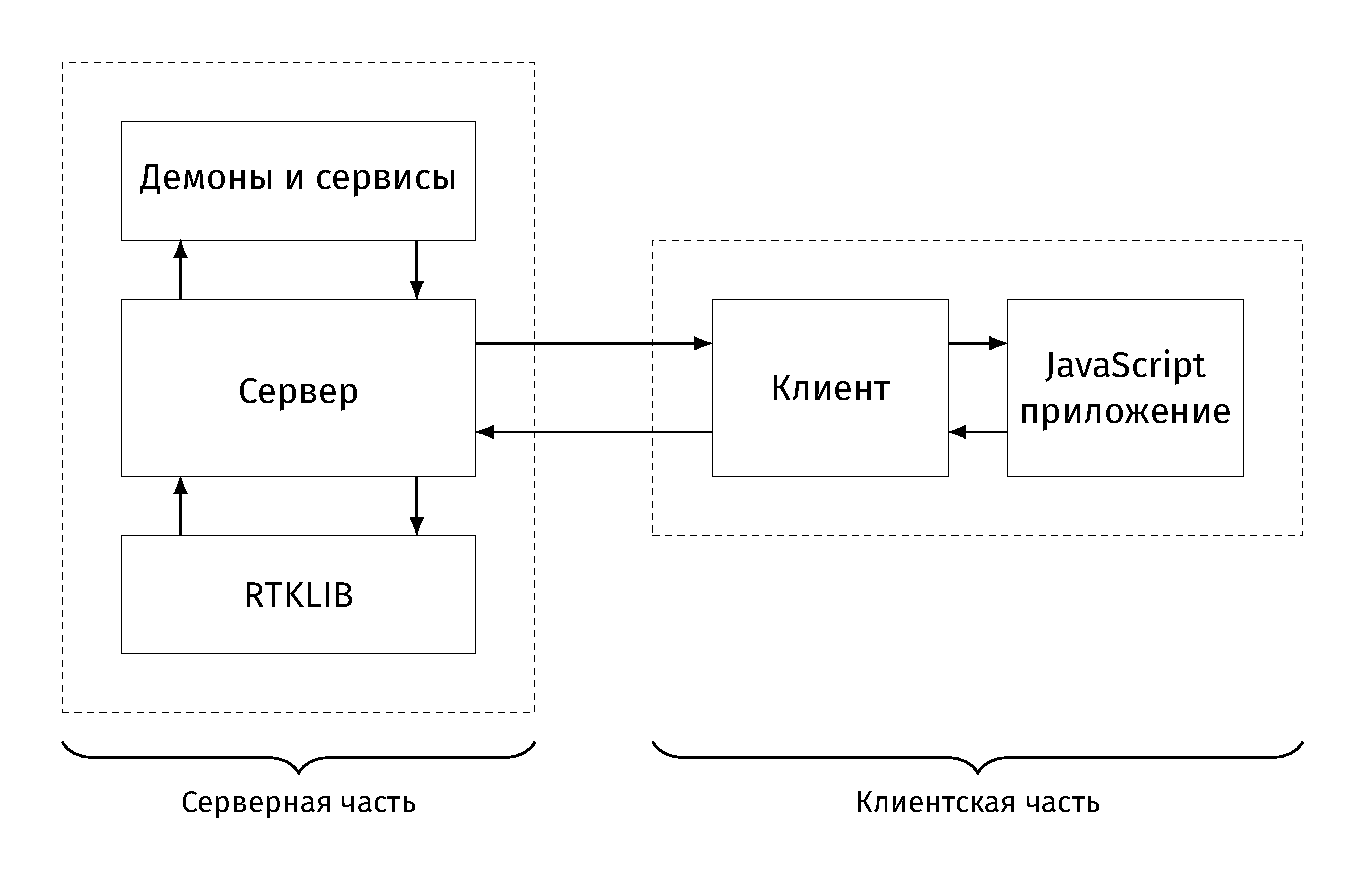
\includegraphics[width=.9\textwidth]{img/tikz/raw-system-architecture/pic}
  \vspace*{12pt}
  \caption{Общая архитектура приложения}\label{fig:raw-system-architecture}
\end{figure}

\subsection{Выбор инструментов разработки}

\subsubsection{Серверная часть приложения}

В~рамках разработки описанного приложения выбор инструментов для написания серверной части приложения зависит не только от возможностей веб-фреймворков, доступных для того или иного языка программирования, но и~от задач, описанных в~подразделе 2.2. Также, важно помнить, что разрабатываемое приложение предназначено для запуска на устройствах с~ограниченными вычислительными ресурсами. \par

Разработчиками серверной части приложения был проведён обзор высокоуровневых языков программирования, часто используемых для разработки веб-приложений. Основными из рассмотренных вариантов были такие популярные языки, как Java, Python, Ruby. \par

% TODO Оформить "переход" к списку наиболее важных библиотек/фреймворков
На основании различных оценок, детали формирования которых выходят за рамки рассматриваемой работы, основным языком для серверной части приложения был выбран Python.

\begin{dashitemize}
  \item Веб-фреймворк Flask
  \item pexpect
  \item GeoPandas
\end{dashitemize}

\subsubsection{Клиентская часть приложения}

% TODO Дополнить содержание + исправить порядок абзацев
Как уже было сказано ранее, клиентскую часть разрабатываемого решения было решено реализовать в~виде одностраничного приложения. \par

Для работы с WebSocket была выбрана библиотека Socket.IO [?]. Данный выбор обусловлен не только популярностью библиотеки, но и наличием полной поддержки Socket.IO на серверной части приложения -- для веб-фреймворка Flask существует расширение Flask-SocketIO, позволяющее серверу обмениваться сообщениями с любыми клиентами Socket.IO.

\begin{dashitemize}
  \item HTML + JavaScript
  \item Vue.js + Vuex
  \item Socket.IO
  \item D3
  \item OpenLayers
\end{dashitemize}

\subsection{Детализированная архитектура приложения}

\subsubsection{Подробная архитектура клиентской части приложения}

\subsection{Создание макета веб-приложения}

\subsubsection{Общий вид приложения}

\subsubsection{Детализация интерфейса отдельных модулей приложения}

\begin{dashitemize}
  \item \textbf{Статус}.
  \item \textbf{Изыскания}.
  \item \textbf{Настройки RTK}.
  \item \textbf{Входящие поправки}.
  \item \textbf{Выдача позиции}.
  \item \textbf{Режим базы}.
  \item \textbf{Логирование}.
  \item \textbf{Управление камерой}.
  \item \textbf{Wi-Fi/Bluetooth}.
  \item \textbf{Настройки}.
\end{dashitemize}

\newpage

  \mysection{РАЗРАБОТКА ПРИЛОЖЕНИЯ}

\subsection{Подготовка окружения для разработки}

Основой разрабатываемого приложения является JavaScript-фреймворк Vue.js. Данный фреймворк позволяет начать работу над проектом максимально просто -- достаточно добавить на веб-страницу JavaScript-файл с~кодом Vue.js, используя тег \,\verb|<script>|.

Однако, для обеспечения удобства разработки и~возможности использования новейших возможностей языка JavaScript было решено использовать пакетный менеджер NPM \cite{NPM} вместе с~компилятором Babel \cite{Babel} и~утилитой Webpack \cite{Webpack}, предназначенной для сборки веб-приложений.


\subsubsection{Пакетный менеджер NPM}

\textbf{NPM} (аббр. \emph{Node Package Manager}) -- менеджер пакетов, входящий в~состав программной платформы Node.js \cite{NodeJS}. NPM существенно упрощает установку компонентов, необходимых для работы или сборки приложения.

При работе с~данным пакетным менеджером, особый интерес представляет файл \textbf{package.json}. Данный файл содержит информацию о~разрабатываемом приложении: название, версия, описание и~т.д (см. листинг \ref{lst:package_json}). Но наиболее важным содержимым файла package.json являются зависимости -- список имён и~версий пакетов, требующихся для работы приложения.


\subsubsection{Babel}

\textbf{Babel} -- транспилер (англ. \emph{transpiler}), транслирующий код JavaScript стандартов ES2015 и~новее \cite{ecma262} в~код более ранних версий JavaScript.

Применение данного инструмента при разработке проекта позволяет использовать возможности JavaScript, представленные в~новейших стандартах языка, не теряя при этом совместимость приложения со~старыми версиями веб-браузеров.

% TODO Пример работы Babel
% TODO Список поддерживаемых браузеров?
\lstinputlisting[
  caption={Пример содержимого файла package.json},
  label={lst:package_json}
]{src/package.json}


\subsubsection{Webpack}

\textbf{Webpack} -- система сборки для JavaScript-приложений, предназначенная, в первую очередь, для генерирования статических ресурсов на основе JavaScript-модулей и~их зависимостей.

Одним из основных преимуществ Webpack является его способность работать с~практически любыми типами ресурсов. Данная возможность обеспечивается дополнительно устанавливаемых \emph{загрузчиков} (англ. \emph{loaders}), которые, к~примеру, позволяют:
\begin{dashitemize}
  \item производить компиляцию JavaScript-файлов с~помощью Babel;
  \item осуществлять статический анализ кода с~помощью ESLint \cite{ESLint};
  \item минифицировать и обфусцировать код приложения;
  \item обрабатывать файлы с~расширением <<.vue>> (однофайловые компоненты Vue.js);
  \item производить трансляцию стилей, описанных на языке SCSS \cite{Sass}, в~CSS.
\end{dashitemize}

Стоит также отметить, что с~помощью Webpack можно существенно облегчить разработку ве-приложения. Благодаря специальным расширениям становится возможно запустить локальный HTTP-сервер, позволяющий просматривать и~отлаживать разрабатываемое приложение в~браузере компьютера, на котором ведётся разработка.



\subsection{Структура проекта. Артефакты сборки (?)}


\subsubsection{Структура проекта}

Исходный код клиентской части приложения является частью Python-проекта, написанного с использованием веб-фреймворка Flask. Подобная структура проекта позволяет держать весь код приложения в одном репозитории и облегчает сборку Python-приложения, предназначенного для установки на устройства Reach и~Reach~RS.

Код клиентского веб-приложения находится в директории \emph{static-src}. Структура данной директории подробно описана на рисунке \ref{fig:project-tree}.

\begin{figure}[h!]
  \centering
  \setlength{\fboxsep}{5pt}
  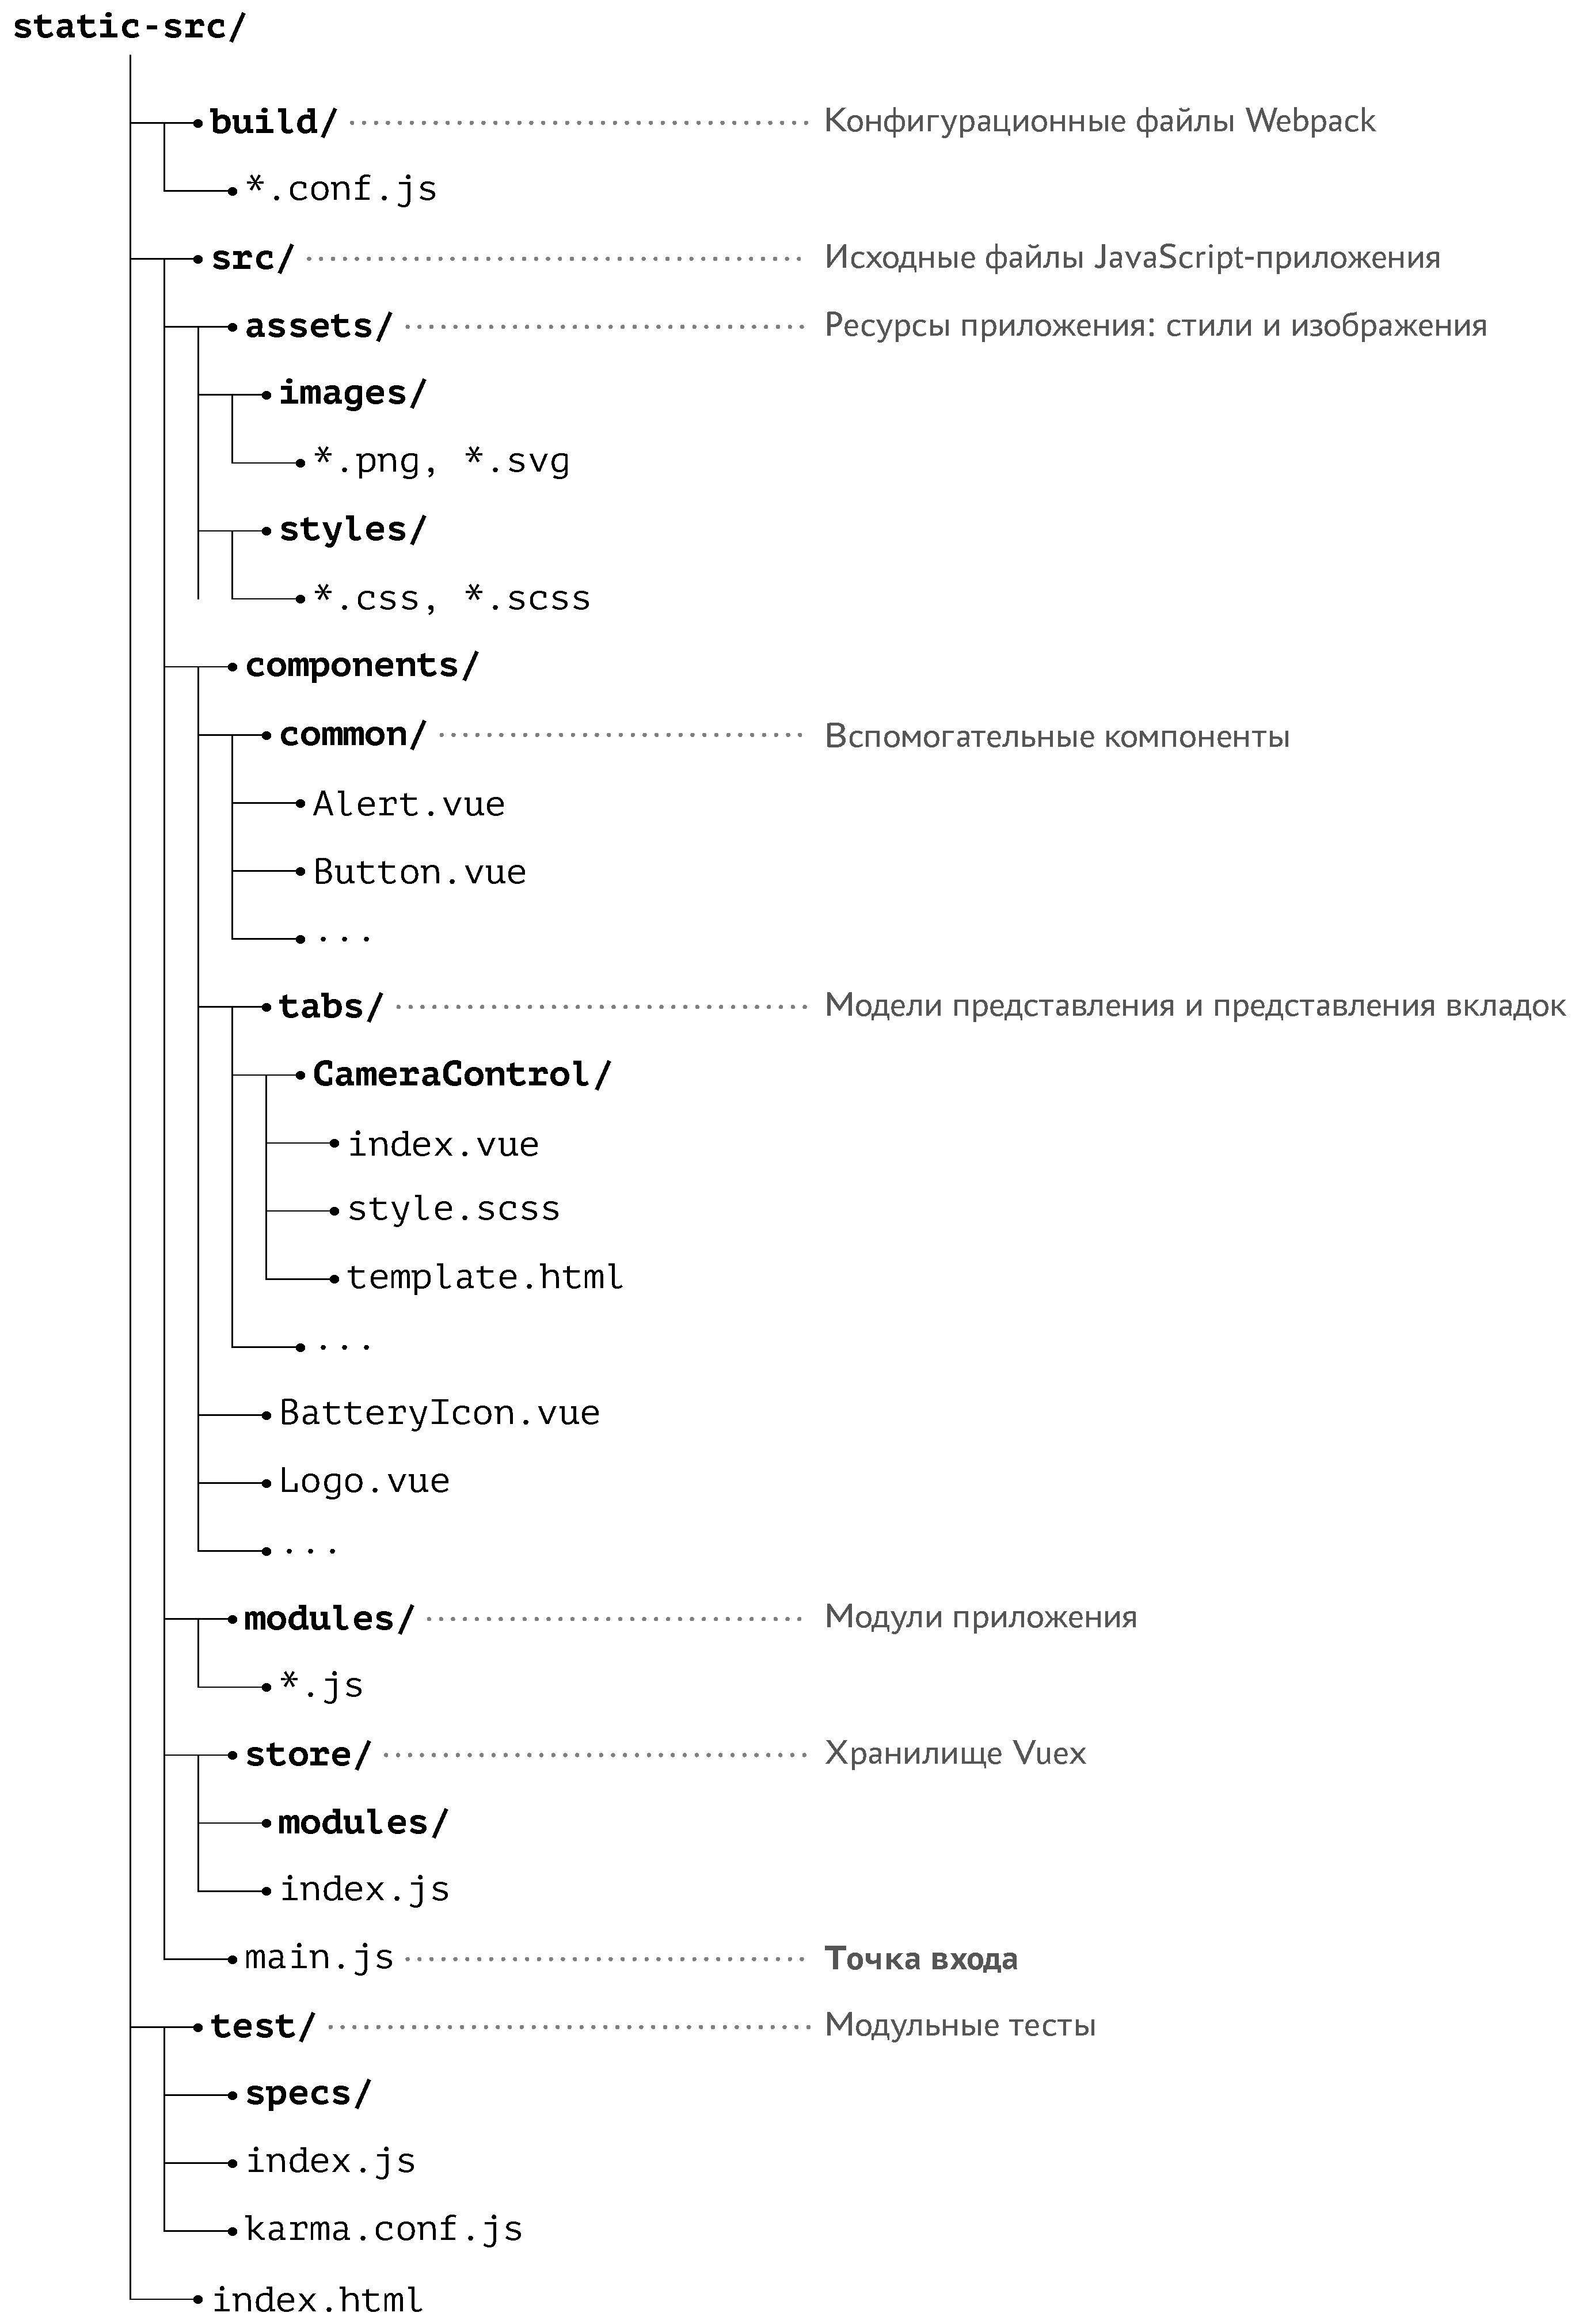
\includegraphics[width=.95\textwidth]{img/tikz/project-tree/pic}
  \vspace*{6pt}
  \caption{Структура проекта}\label{fig:project-tree}
\end{figure}


\subsubsection{Точка входа}


\subsubsection{Артефакты сборки}



\subsection{Глобальное хранилище данных приложения. Однонаправленный поток данных}

\textbf{Vuex} -- библиотека-расширение для Vue.js приложений, позволяющая создавать глобальное хранилище данных, доступное для всех модулей и Vue-компонентов, входящих в~состав проекта. Подобное хранилище необходимо не только для обмена данными между компонентами -- основной его задачей является управление состоянием представлений приложения.

Идеи, лежащие в~основе данной библиотеки, унаследованы от архитектуры Flux \cite{Flux}. Vuex предоставляет шаблонный подход к~управлению состояниями компонентов приложения, основанный на \emph{однонаправленном потоке данных}.


\subsubsection{Однонаправленный поток данных}

Взаимный обмен данными и~событиями между моделями и~представлениями при наличии большого числа компонентов является потенциальным источником ошибок. Асинхронные изменения и~побочные эффекты могут существенно усложнить разработку и~отладку, а~также нарушить работу приложения.

% TODO Добавить "переход" к этому абзацу
Однонаправленный поток данных в~простейшем виде представлен на рисунке \ref{fig:simple-oneway-data-flow}.

\begin{figure}[h!]
  \centering
  \setlength{\fboxsep}{5pt}
  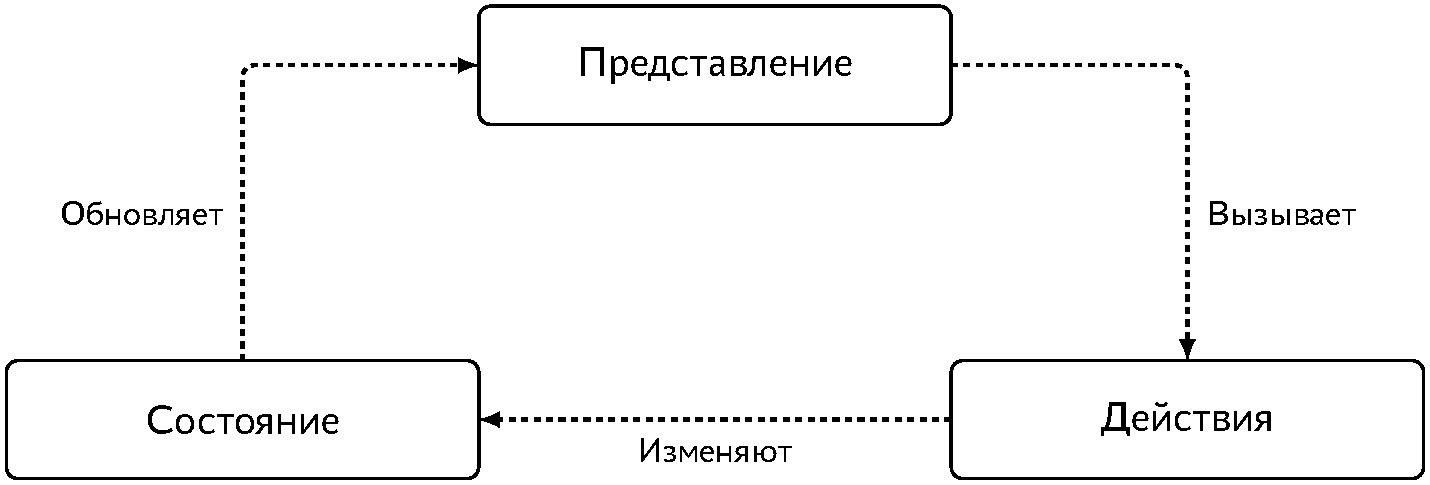
\includegraphics[width=.9\textwidth]{img/tikz/simple-oneway-data-flow/pic}
  \vspace*{12pt}
  \caption{Однонаправленный поток данных}\label{fig:simple-oneway-data-flow}
\end{figure}

Подход, описанный на рисунке \ref{fig:simple-oneway-data-flow}, прекрасно подходит для управления представлением одного компонента. Однако, при появлении нескольких компонентов, зависящих от одного и~того же состояния, структура приложения может существенно усложниться.

% TODO Сноска про <<одиночку>>?
Vuex решает проблему, описанную выше, вводя в~структуру приложения глобальное хранилище данных, являющееся состоянием-<<одиночкой>> (англ. \emph{singleton}), которое обновляет все необходимые представления с~помощью реактивных обновлений.

Для избежания неконтролируемых изменений состояния в~Vuex введено следующее ограничение: изменить состояние можно только с~помощью синхронных транзакций, называемых \emph{мутациями}.

Асинхронные операции, результаты выполнения которых изменяют состояние, в~Vuex получили название \emph{<<действия>>}. Внутри функций-обработ-чиков действий становится возможно, к~примеру, совершить асинхронный запрос к~серверу, а~при получении результата сделать одну или более синхронных мутаций состояния.

Схема организации однонаправленного потока данных при использовании Vuex изображена на рисунке \ref{fig:vuex-oneway-data-flow}.

\begin{figure}[h!]
  \centering
  \setlength{\fboxsep}{5pt}
  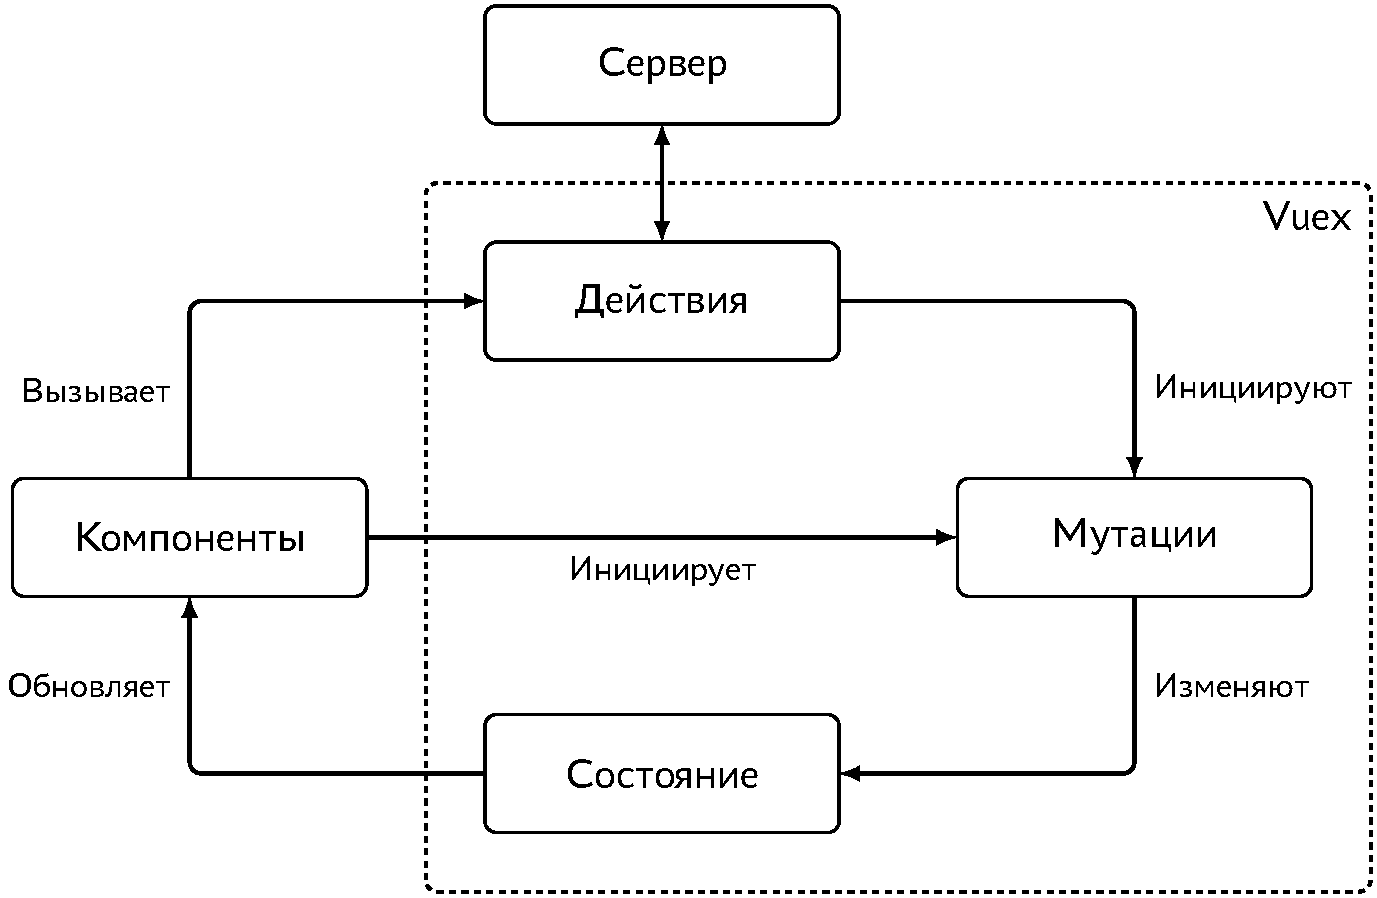
\includegraphics[width=.9\textwidth]{img/tikz/vuex-oneway-data-flow/pic}
  \vspace*{12pt}
  \caption{Однонаправленный поток данных при использовании Vuex}\label{fig:vuex-oneway-data-flow}
\end{figure}


\subsubsection{Модули хранилища данных}

Глобальные данные о~состоянии приложения по умолчанию хранятся в~одном и~том же объекте. Рост числа модулей приложения неизбежно приводит к~тому, что структура данного объекта существенно усложняется, а~именование мутаций и~действий может вызывать затруднения из-за требования к~уникальности имён сущностей Vuex.

Для решения описанных выше проблем Vuex предоставляет инструменты для разделения хранилища на \emph{модули}. Модули представляют из себя самостоятельные части глобального состояния, каждая из которых может содержать объект с~данными, мутации и~т.д. При использовании данного подхода возможные проблемы с~именованием решаются благодаря тому, что каждый модуль Vuex может иметь собственное пространство имён.

% TODO Добавить пример работы с модулями

Хранилище Vuex, используемое в разрабатываемом приложении, было разделено на модули, соответствующие важнейшим подсистемам программного обеспечения устройств Reach и~Reach~RS:
\begin{dashitemize}
  \item позиционирование и~режим RTK;
  \item конфигурация устройства;
  \item входящие и~исходящие потоки данных;
  \item состояние компонентов графического интерфейса.
\end{dashitemize}

Схема модулей глобального хранилища, используемого в~приложении, изображена на рисунке \ref{fig:vuex-modules}.

\begin{figure}[h!]
  \centering
  \setlength{\fboxsep}{5pt}
  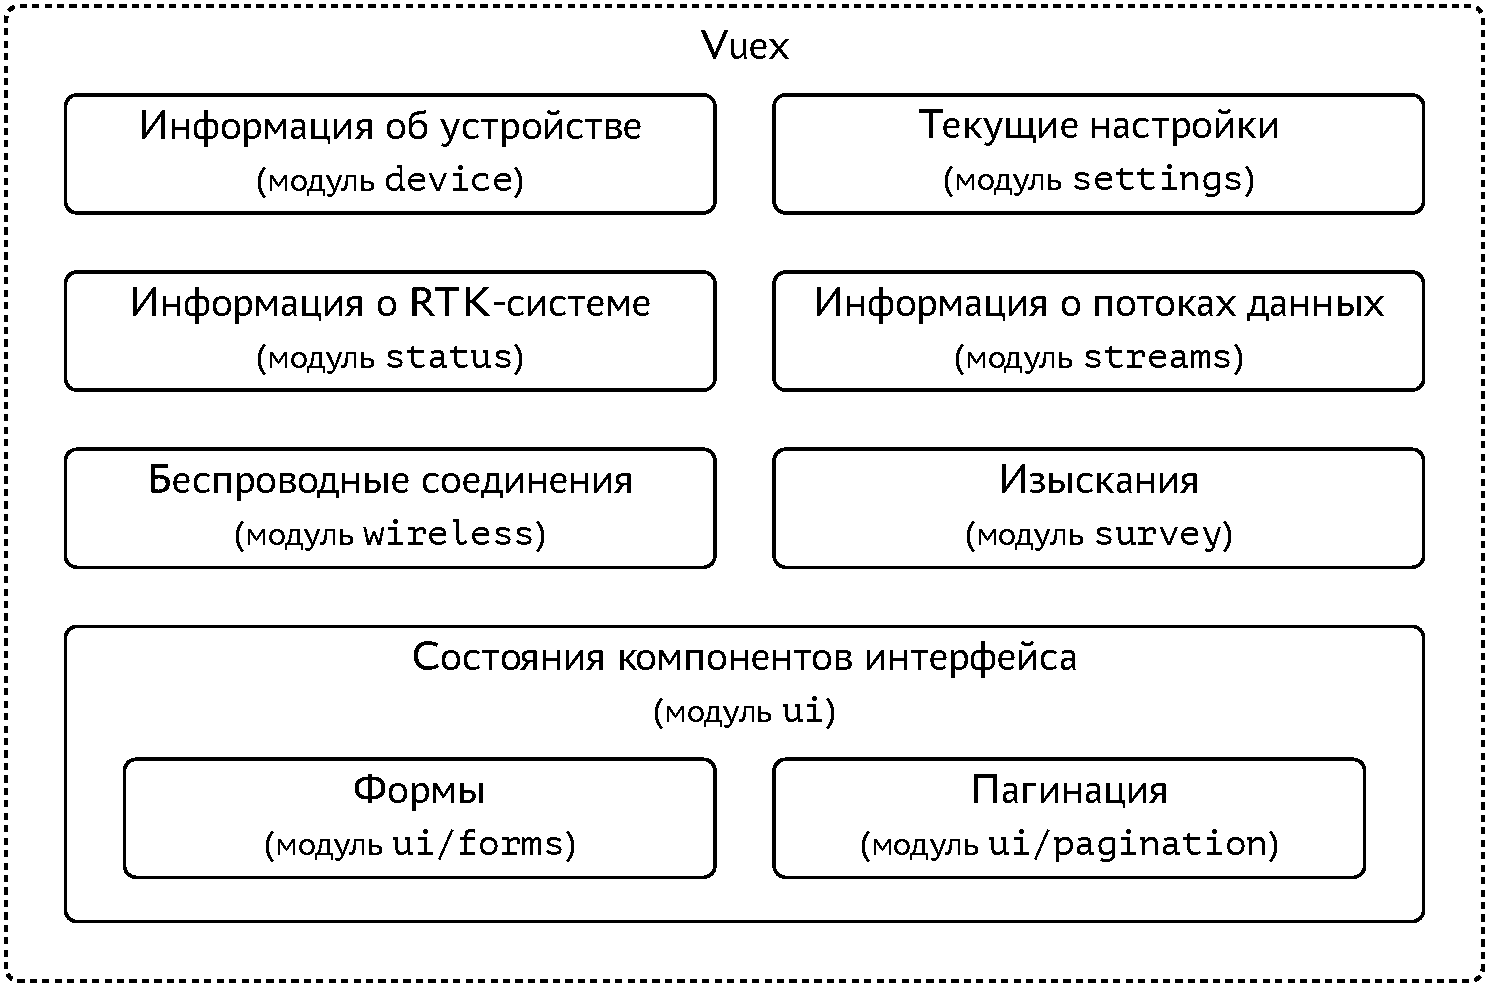
\includegraphics[width=.9\textwidth]{img/tikz/vuex-modules/pic}
  \vspace*{6pt}
  \caption{Модульная структура хранилища Vuex}\label{fig:vuex-modules}
\end{figure}



\subsection{Модули и~компоненты приложения}

В пунктах, следующих далее, описана структура и~организация модулей и~компонентов разрабатываемого веб-приложения. Первые два пункта посвящены модулям общего назначения и~вспомогательным компонентам, которые необходимы для создания моделей представления, описанных в~подразделе \ref{subsec:app-modules-requirements}. Сами же модели представления описаны в~третьем пункте текущего подраздела.


\subsubsection{Модули общего назначения}

К~модулям общего назначения относятся модуль работы с~картами и~модуль обработки событий. Рассмотрим каждый из их подробнее.

\paragraph{Модуль работы с~картами}

Модуль работы с~картами представляет из себя обёртку (англ. \emph{wrapper}) над частью библиотеки OpenLayers, используемой в~разрабатываемом приложении для отображения карт и различной информации на них. Код модуля содержится в~файле \emph{olWrapper.js}.

Данный модуль предназначен для повышения удобства создания однотипных карт -- для добавления карты на определённую страницу достаточно импортировать модуль в нужную часть кода приложения и~вызвать соответствующие функции.

Импорт необходимых модулей OpenLayers, единожды осуществляемый в~модуле работы с~картами (см.~листинг \ref{lst:modules__maps__imports}), исключает повторение существенного количества строк кода и~уменьшает размер файла vendor.js.

\lstinputlisting[
  caption={olWrapper.js: импорт необходимых модулей OpenLayers},
  label={lst:modules__maps__imports}
]{src/modules__maps__imports.js}

% TODO Добавить полный листинг в Приложения


\paragraph{Модуль обработки событий}

Модуль обработки событий (\emph{eventsModule.js}) выполняет ряд ключевых задач, необходимых для работы приложения:
\begin{dashitemize}
  \item инициализация WebSocket-подключения;
  \item обработка разрыва (восстановления) соединения с сервером;
  \item оповещение пользователя о различных событиях.
  \item инициализация модулей Vuex путём вызова их действий.
\end{dashitemize}

В листинге \ref{lst:modules__events__short} представлено содержимое файла eventsModule.js (полный листинг файла см. в приложении ??). По умолчанию модуль экспортирует функцию, выполнение которой зарегистрирует несколько слушателей событий Socket.IO и вызовет действие \emph{<<activate>>} (\emph{activate} с англ. -- <<активировать>>) в четырёх модулях Vuex.

Действия с названием <<activate>> присутствуют во всех модулях Vuex, кроме модулей, отвечающих за хранение состояния компонентов интерфейса (см. рис.~\ref{fig:vuex-modules}). <<Активация>> модуля Vuex подразумевает под собой:
\begin{dashitemize}
  \item установка значений по умолчанию в объекте состояния (при необходимости);
  \item регистрация слушателей определённых широковещательных сообщений сервера;
  \item отправка на сервер запросов на получение данных;
  \item создание таймеров для периодических опросов сервера.
\end{dashitemize}

\lstinputlisting[
  caption={Модуль обработки событий},
  label={lst:modules__events__short}
]{src/modules__events__short.js}

Также модуль обработки событий экспортирует объект \emph{socket}, импортируя который, любой компонент приложения сможет осуществлять общение с сервером через WebSocket-события.


\subsubsection{Вспомогательные компоненты}

Вспомогательные компоненты представляют из себя набор блоков и элементов интерфейса, необходимых для создания всевозможных представлений приложения. Данные компоненты включают в себя кнопки, переключатели, панели, индикаторы выполнения и т.д.


\subsubsection{Модели представления}

\paragraph{Статус}

\paragraph{Изыскания}

\paragraph{Модули настройки параметров работы устройства}

\paragraph{Модули настройки входящих и исходящих потоков данных}

\paragraph{Модули настройки беспроводных соединений}

\paragraph{Общие настройки}

\newpage

  \mysection{АПРОБАЦИЯ РЕЗУЛЬТАТОВ РАЗРАБОТКИ}

\subsection{Установка приложения на модули и приёмники}

Разработанный пользовательский веб-интерфейс в~составе Python-при-ложения был установлен на несколько устройств Reach и~Reach~RS. Автором работы совместно с~разработчиками серверной части приложения было произведено ручное тестирование всех представлений и~форм, доступных через веб-приложение.

Работа приложения была протестирована на различных устройствах, работающих под управлением ОС семейства Windows, macOS, Linux, а~также на нескольких версиях мобильных систем Android и~iOS.

Была проверена доступность приложения при подключении приёмников к~Wi-Fi-сетям в~качестве клиента, а~также при их работе в~режиме точки доступа.



\subsection{Полевые испытания устройств}

Разработанный веб-интерфейс был протестирован при работе устройств под открытым небом. Проверено поведение приложения при:
\begin{dashitemize}
  \item отключении и~подключении антенны во~время работы устройства (для модулей Reach);
  \item потере и восстановлении соединения с~базой;
  \item намеренном добавлении помех к~сигналам, получаемым устройством со~спутников.
\end{dashitemize}

При тестировании устройств под открытым небом особое внимание было уделено проверке раздела <<Изыскания>>. Был произведён ручной сбор точек на местности, а~также осуществлена проверка работы приложения при использовании правил автоматического сбора точек.



\subsection{Бета-версии приложения}

С конце 2016 года было начато распространение бета-версии разработанного веб-приложения. Установка данного приложения подразумевала перепрошивку устройства.

Благодаря инициативной группе опытных геодезистов, являющихся пользователями устройств Reach, были собраны отчёты о~найденных ошибках и пожелания по доработке приложения.

В~настоящее время приложение стало основной рабочей версией веб-интерфейса для Reach и~Reach~RS.



\subsection{Выводы по разделу 4}

\begin{dashitemize}
  \item По окончании процесса разработки все функции веб-приложения были протестированы автором работы и~сотрудниками компании Emlid.
  \item Работа приложения была протестирована в~веб-браузерах нескольких устройств, работающих под управлением различных операционных систем.
  \item Были проведены испытания приложения при работе с~устройствами под открытым небом.
  \item Бета-версии приложения были протестированы инициативной группой пользователей, имеющих опыт работы с~профессиональным геодезическим оборудованием.
  \item Разработанное приложение было успешно внедрено в~качестве основной рабочей версии веб-интерфейса устройств Reach и Reach~RS.
\end{dashitemize}

\newpage
  \mysection*{ЗАКЛЮЧЕНИЕ}

В рамках проведённой работы были получены следующие результаты:
\begin{dashitemize}
  \item Проведён обзор областей применения высокоточного позиционирования. Были рассмотрены проблемы доступности профессионального геодезического оборудования и~распространённости открытого программного комплекса высокоточного позиционирования RTKLIB.
  \item Проведён анализ применения веб-интерфейсов для взаимодействия с~устройствами без органов управления.
  \item Сформулированы требования к~созданию веб-приложения для взаимодействия с~устройствами Reach и~Reach~RS компании Emlid, работающими под под управление программного обеспечения, работающего на основе пакета RTKLIB.
  \item Создана детализированная архитектура приложения, на основе которой было разработано веб-приложение, полностью удовлетворяющее всем заявленным требованиям.
  \item Для приложения созданы комплексы модульных и~функциональных текстов, позволяющие автоматизировать проверку работоспособности приложения.
  \item Проведена апробация результатов работы. Устройства, с~установленным на них разработанным веб-приложением, были протестированы сотрудниками компании Emlid, а~также инициативной группой опытных геодезистов, пользующихся устройствами Reach и~Reach~RS.
  \item На основе полученных в~ходе апробации отчётах об ошибках и~пожеланиях произведены доработки приложения. Разработанный продукт был успешно внедрён в~качестве основной рабочей версии веб-интерфейса для устройств Reach и~Reach~RS.
\end{dashitemize}

\newpage

Автор планирует продолжать работу над проектом и~развивать его, добавляя новые функции и~исправляя возможные ошибки, которые могут быть найдены во время эксплуатации приложения.

\newpage

  % %!TEX root = ../main.tex

\mysection*{СПИСОК ТЕРМИНОВ}

\renewcommand{\descriptionlabel}[1]{%
  \hspace\labelsep \upshape\bfseries #1:%
}

\begin{description}
  \item[IRR] Internal Rate of Return
  \item[NPV] Net Present Value
  \item[PPP] Purchasing Power Parity
\end{description}

\newpage


  \phantomsection
  \addcontentsline{toc}{section}{Библиографический список}

  \hyphenpenalty=10000
  \interlinepenalty=10000

  \nocite{*}
  \bibliography{biblio}
  
  \clearpage
  
  \begin{appendices}
    \mysection{}

hello

\clearpage
    \section{}
\label{sec:appendix_events-module}

\lstinputlisting[
  title={Листинг Б.1 -- Тесты для компонента <<переключатель>>},
  label={lst:test__toggle}
]{src/test__toggle.js}

\clearpage

  \end{appendices}
\end{document}
